%! TeX program = lualatex
\documentclass{scrartcl}
\usepackage[left=4cm,right=3cm,top=3cm,bottom=3cm, marginpar=3cm]{geometry}
\setlength{\parindent}{0pt}
\setlength{\parskip}{1ex}

\usepackage{cprotect}
\usepackage{tikz}
\usetikzlibrary{math}

\usepackage{xcolor}
\usepackage{soul}

\usepackage{hyperref}
\hypersetup{
    pdftitle={Easy colorblind-safe typesetting: the colorblind package},
    pdfauthor={Simon Pfahler},
}
\usepackage{cleveref}

\usepackage{csquotes}
\usepackage[backend=biber, style=numeric-comp, seconds=true, sorting=none, subentry=true, doi=false, alldates=iso]{biblatex}
\renewcommand*{\entrysetpunct}{\\[5pt]}
\addbibresource{bib.bib}

\usepackage[Tol, OkabeIto]{colorblind}

\newcommand\colorblind{\textbf{colorblind} }
\newcommand\hlc[2][T-Q-PH4]{{%
    \colorlet{foo}{#1}%
    \sethlcolor{foo}\hl{#2}}%
}

\reversemarginpar
\newcommand\marg[1]{\leavevmode\marginpar{\raggedleft #1}}
\newcommand\tbs{\textbackslash}

\title{Easy colorblind-safe typesetting:\\ the \colorblind package}
\author{Simon Pfahler}
\date{\today\\Version 0.1}


\begin{document}

\maketitle

\begin{abstract}
    In colorblind-safe documents, the contents are presented in a way that the same information is conveyed to readers regardless of a potential color vision deficiency.
    This package provides the tools necessary for color-agnostic typesetting in \LaTeX.
    It provides color schemes for a wide range of applications.
    The most commonly used schemes are qualitative schemes, providing easily distinguishable colors for use in graphics, but also for text coloring or highlighting.
    Additionally, diverging and sequential schemes are included which can be used for encoding quantitative information in the colors of a graphic.
    Therefore, colorblind-safeness is incorporated into the writing process, making it both less cumbersome and less error-prone.
\end{abstract}

\tableofcontents
\clearpage

\section{Introduction}
\cprotect\marg{\verb!Tol!\\\verb!OkabeIto!}%
The \colorblind package provides the color schemes by Paul Tol~\cite{Tol} and the Okabe Ito color palette~\cite{Ichihara_2008}.
By default, no schemes are loaded.
Providing one of the options \verb!Tol! or \verb!OkabeIto! loads all corresponding schemes.

As an example for how to use the colors, we look at the \emph{bright qualitative} color scheme by Tol.
\cref{fig:T-Q-Bexample} shows the colors in the scheme

\begin{figure}[ht]
    \centering
    \drawScheme{T-Q-B}
    \caption{Bright qualitative color scheme by Tol.}
    \label{fig:T-Q-Bexample}
\end{figure}

All colors in this model start with \verb!T-Q-B!, indicating that it is a scheme by \textbf{T}ol, that it is a \textbf{q}ualitative scheme, and that it is the \textbf{b}right scheme.
The colors in the scheme are specified by a number following the scheme name, in this case ranging from \verb!T-Q-B1! to \verb!T-Q-B6! for the non-grey colors.
The additional color \verb!T-Q-B0! provides a color that can be used, e.g., to indicate bad data.

There are two reasons why color names are not based on natural color names (e.g., \hlc[T-Q-PH1]{blue}):
\begin{enumerate}
    \item Certain colors (\hlc[T-Q-PH3]{green}, \hlc[T-Q-PH5]{red}) are often used by people with full color vision to convey certain meanings (\hlc[T-Q-PH3]{good}, \hlc[T-Q-PH5]{bad}).
        This meaning is difficult for people with color-deficiencies to pick up.
        By not using natural color names, it is easier to write color-agnostic documents that do not make use of said connotations.
    \item Natural color names can be cumbersome, e.g., when multiple variations of \hlc[T-Q-PH1]{blue} are used. It is annoying having to look up if a color is called, e.g., \hlc[T-Q-PH1]{light blue} or \hlc[T-Q-PH2]{cyan}.
\end{enumerate}

These colors are used the same way as any other colors. To change the text color to \verb!T-Q-B1! for example, use \verb!\color{T-Q-B1}!.

\section{Guidelines}
On its own, using colorblind-safe colors is not sufficient for making a document truly colorblind-safe.
This section provides some general rules to follow for colorblind-safe typesetting.

These rules apply to each visual unit of a document individually.
A visual unit may be a graphic, a table or a paragraph of text.
It might be advisable to be consistent also between different visual units (e.g., use the same color scheme for all graphics), but this is more of an aesthetic argument and is not necessary for a colorblind-safe document.

The most important rules are, in this order:
\begin{enumerate}
    \item \hlc{Do not mix the colors in qualitative schemes!}\newline
        Mixing of colors, e.g., \verb?T-Q-B1!50!T-Q-B5? also interferes with the packages intention of providing distinguishable colors.
    \item \hlc{Only use colors from one color scheme for a given visual unit!}\newline
        The colors are defined with the purpose of being easily distinguishable, but this is only true within each color scheme.
        Using colors from multiple schemes therefore defies the point of this package.
    \item \hlc{Do not use shades of colors!}\newline
        Saturation and brightness are also used for distinguishability, so mixings involving \verb!white! and \verb!black! should also be avoided.
\end{enumerate}

The first two rules should be ensured in any visual unit. If the need for more colors arises, a different color scheme should be used alltogether.
While the third rule should also be followed in most scenarios, there are some situations that might allow for breaking this rule. As an example, consider \cref{fig:errorbar_plot}, where the error band is colored with a lighter shade of the original color.

\begin{figure}[ht]
    \centering
    \includegraphics{Graphics/errorbar_plot/errorbar_plot.pdf}
    \cprotect\caption{This plot breaks rule 3 by using the shade \verb?T-Q-B5!20? for the error band of the reference.}
    \label{fig:errorbar_plot}
\end{figure}

There are additional guidelines that should be kept in mind when typesetting colorblind-safe documents.
Depending on the specific visual unit, they are usually not as vital as the rules stated above.
In no particular order, they are:
\begin{itemize}
    \item \hlc{Do not convey information only through color!}\newline
        When possible, encode the information the color provides also in a different way, e.g., through text, patterns or symbols.
    \item \hlc{Do not use color for information and aesthetics simultaneously!}\newline
        Color is often also used for aesthetic reasons, e.g., on a scientific poster.
        While this is ok in principle, do not mix information and aesthetics within the same visual unit, as this makes it more difficult to extract the encoded information.
\end{itemize}

\section{Provided color schemes}\label{sec:colors}

\subsection{Paul Tol's color schemes}

\subsubsection{Qualitative color schemes}

\begin{figure}[ht]
    \centering
    \drawScheme{T-Q-B}
    \caption{Bright qualitative color scheme by Paul Tol~\cite{Tol}.}
    \label{fig:T-Q-B}
\end{figure}

\begin{figure}[ht]
    \centering
    \drawScheme{T-Q-HC}
    \caption{High-contrast qualitative color scheme by Paul Tol~\cite{Tol}.}
    \label{fig:T-Q-HC}
\end{figure}

\begin{figure}[ht]
    \centering
    \drawScheme{T-Q-V}
    \caption{Vibrant qualitative color scheme by Paul Tol~\cite{Tol}.}
    \label{fig:T-Q-V}
\end{figure}

\begin{figure}[ht]
    \centering
    \drawScheme{T-Q-M}
    \caption{Muted qualitative color scheme by Paul Tol~\cite{Tol}.}
    \label{fig:T-Q-M}
\end{figure}

\begin{figure}[ht]
    \centering
    \drawScheme{T-Q-MC}
    \caption{Medium-contrast qualitative color scheme by Paul Tol~\cite{Tol}.}
    \label{fig:T-Q-MC}
\end{figure}

\begin{figure}[ht]
    \centering
    \drawScheme{T-Q-PH}
    \caption{Pale qualitative color scheme by Paul Tol~\cite{Tol}, for highlighting only.}
    \label{fig:T-Q-PH}
\end{figure}

\begin{figure}[ht]
    \centering
    \drawScheme{T-Q-DT}
    \caption{Dark qualitative color scheme by Paul Tol~\cite{Tol}, for text color only.}
    \label{fig:T-Q-DT}
\end{figure}

\begin{figure}[ht]
    \centering
    \drawScheme{T-Q-L}
    \caption{Light qualitative color scheme by Paul Tol~\cite{Tol}.}
    \label{fig:T-Q-L}
\end{figure}

\subsubsection{Diverging color schemes}

\begin{figure}[ht]
    \centering
    \drawScheme{T-D-S}
    \caption{Sunset diverging color scheme by Paul Tol~\cite{Tol}.}
    \label{fig:T-D-S}
\end{figure}

\begin{figure}[ht]
    \centering
    \drawScheme{T-D-BR}
    \caption{BuRd diverging color scheme by Paul Tol~\cite{Tol}.}
    \label{fig:T-D-BR}
\end{figure}

\begin{figure}[ht]
    \centering
    \drawScheme{T-D-PG}
    \caption{PRGn diverging color scheme by Paul Tol~\cite{Tol}.}
    \label{fig:T-D-PG}
\end{figure}

\subsubsection{Sequential color schemes}

\begin{figure}[ht]
    \centering
    \drawScheme{T-S-YB}
    \caption{YlOrBr sequential color scheme by Paul Tol~\cite{Tol}.}
    \label{fig:T-S-YB}
\end{figure}

\begin{figure}[ht]
    \centering
    \drawScheme{T-S-DR}
    \caption{Discrete Rainbow sequential color scheme by Paul Tol~\cite{Tol}.}
    \label{fig:T-S-DR}
\end{figure}

\subsection{Okabe Ito qualitative color scheme}

\begin{figure}[ht]
    \centering
    \drawScheme{OI}
    \caption{Okabe Ito qualitative color scheme~\cite{Ichihara_2008}.}
    \label{fig:OI}
\end{figure}

\subsection{Provided commands}
\cprotect\marg{\verb!\drawScheme{...}!}%
The visualizations of color schemes given in this documentation are created with the command \verb!\drawScheme{...}!.
Only the prefix of a color scheme should be provided to the command, e.g.\ \verb!\drawScheme{T-Q-B}! to print the qualitative bright scheme by Tol, as can be seen in \cref{fig:T-Q-B}.


\section{Experimental and work in progress}

\let\oldcolor\color

\newcommand\normalvision{%
    \protect\renewcommand\color[1]{\oldcolor{##1}}%
}

\newcommand\protanopia{%
    \protect\renewcommand\color[1]{%
        \extractcolorspecs{##1}{\modelspec}{\colorspec}%
        \tikzmath{
            \r = array({\colorspec},0);
            \g = array({\colorspec},1);
            \b = array({\colorspec},2);
            \rp = pow(0.06425 + 0.677*pow(\g, 2.2) + 0.2802*pow(\r, 2.2), 1./2.2);
            \gp = pow(0.06425 + 0.677*pow(\g, 2.2) + 0.2802*pow(\r, 2.2), 1./2.2);
            \bp = pow(0.06425 + 0.95724*pow(\b, 2.2) + 0.02138*pow(\g, 2.2) - 0.02138*pow(\r, 2.2), 1./2.2);
        }%
        \oldcolor[rgb]{\rp,\gp,\bp}%
    }%
}

\newcommand\deuteranopia{%
    \protect\renewcommand\color[1]{%
        \extractcolorspecs{##1}{\modelspec}{\colorspec}%
        \tikzmath{
            \r = array({\colorspec},0);
            \g = array({\colorspec},1);
            \b = array({\colorspec},2);
            \rp = pow(0.01194 + 0.8806*pow(\g, 2.2) + 0.1115*pow(\r, 2.2), 1./2.2);
            \gp = pow(0.01194 + 0.8806*pow(\g, 2.2) + 0.1115*pow(\r, 2.2), 1./2.2);
            \bp = pow(0.01194 + 0.992052*pow(\b, 2.2) - 0.003974*pow(\g, 2.2) + 0.003974*pow(\r, 2.2), 1./2.2);
        }%
        \oldcolor[rgb]{\rp,\gp,\bp}%
    }%
}

\begin{figure}[ht]
    \centering
    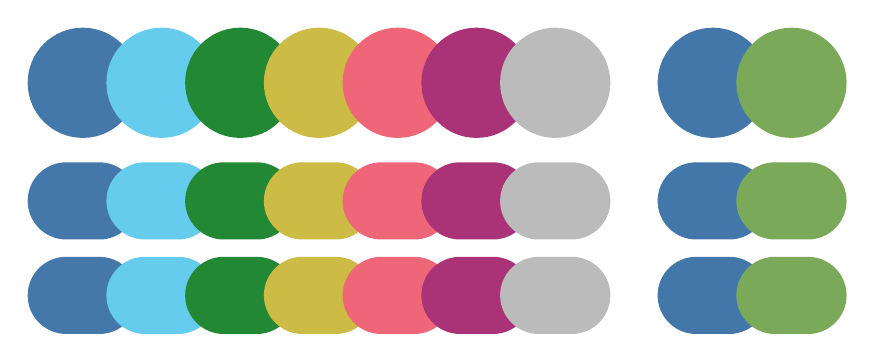
\begin{tikzpicture}
        \newcommand{\dx}{1}
        \newcommand{\dy}{-1.5}
        \newcommand{\radius}{0.7}

        % test for non rgb color models
        \definecolor{hsbtest1}{rgb}{0.266, 0.465, 0.664}
        \definecolor{hsbtest2}{hsb}{0.266, 0.468, 0.664}
        
        % Tol's bright qualitative color scheme
        \fill[T-Q-B1] (0,0) circle (\radius);
        \fill[T-Q-B2] (\dx,0) circle (\radius);
        \fill[T-Q-B3] (2*\dx,0) circle (\radius);
        \fill[T-Q-B4] (3*\dx,0) circle (\radius);
        \fill[T-Q-B5] (4*\dx,0) circle (\radius);
        \fill[T-Q-B6] (5*\dx,0) circle (\radius);
        \fill[T-Q-B0] (6*\dx,0) circle (\radius);

        \fill[hsbtest1] (8*\dx,0) circle (\radius);
        \fill[hsbtest2] (9*\dx,0) circle (\radius);
        
        {
        \protanopia
        \fill[T-Q-B1, rounded corners=0.7*\radius cm]
            (0-\radius,\dy-0.7*\radius) rectangle ++(2*\radius, 1.4*\radius);
        \fill[T-Q-B2, rounded corners=0.7*\radius cm]
            (\dx-\radius,\dy-0.7*\radius) rectangle ++(2*\radius, 1.4*\radius);
        \fill[T-Q-B3, rounded corners=0.7*\radius cm]
            (2*\dx-\radius,\dy-0.7*\radius) rectangle ++(2*\radius, 1.4*\radius);
        \fill[T-Q-B4, rounded corners=0.7*\radius cm]
            (3*\dx-\radius,\dy-0.7*\radius) rectangle ++(2*\radius, 1.4*\radius);
        \fill[T-Q-B5, rounded corners=0.7*\radius cm]
            (4*\dx-\radius,\dy-0.7*\radius) rectangle ++(2*\radius, 1.4*\radius);
        \fill[T-Q-B6, rounded corners=0.7*\radius cm]
            (5*\dx-\radius,\dy-0.7*\radius) rectangle ++(2*\radius, 1.4*\radius);
        \fill[T-Q-B0, rounded corners=0.7*\radius cm]
            (6*\dx-\radius,\dy-0.7*\radius) rectangle ++(2*\radius, 1.4*\radius);

        \fill[hsbtest1, rounded corners=0.7*\radius cm]
            (8*\dx-\radius,\dy-0.7*\radius) rectangle ++(2*\radius, 1.4*\radius);
        \fill[hsbtest2, rounded corners=0.7*\radius cm]
            (9*\dx-\radius,\dy-0.7*\radius) rectangle ++(2*\radius, 1.4*\radius);

        }
        
        {
        \deuteranopia
        \fill[T-Q-B1, rounded corners=0.7*\radius cm]
            (0-\radius,1.8*\dy-0.7*\radius) rectangle ++(2*\radius, 1.4*\radius);
        \fill[T-Q-B2, rounded corners=0.7*\radius cm]
            (\dx-\radius,1.8*\dy-0.7*\radius) rectangle ++(2*\radius, 1.4*\radius);
        \fill[T-Q-B3, rounded corners=0.7*\radius cm]
            (2*\dx-\radius,1.8*\dy-0.7*\radius) rectangle ++(2*\radius, 1.4*\radius);
        \fill[T-Q-B4, rounded corners=0.7*\radius cm]
            (3*\dx-\radius,1.8*\dy-0.7*\radius) rectangle ++(2*\radius, 1.4*\radius);
        \fill[T-Q-B5, rounded corners=0.7*\radius cm]
            (4*\dx-\radius,1.8*\dy-0.7*\radius) rectangle ++(2*\radius, 1.4*\radius);
        \fill[T-Q-B6, rounded corners=0.7*\radius cm]
            (5*\dx-\radius,1.8*\dy-0.7*\radius) rectangle ++(2*\radius, 1.4*\radius);
        \fill[T-Q-B0, rounded corners=0.7*\radius cm]
            (6*\dx-\radius,1.8*\dy-0.7*\radius) rectangle ++(2*\radius, 1.4*\radius);
        
        \fill[hsbtest1, rounded corners=0.7*\radius cm]
            (8*\dx-\radius,1.8*\dy-0.7*\radius) rectangle ++(2*\radius, 1.4*\radius);
        \fill[hsbtest2, rounded corners=0.7*\radius cm]
            (9*\dx-\radius,1.8*\dy-0.7*\radius) rectangle ++(2*\radius, 1.4*\radius);
        }
    \end{tikzpicture}
    \caption{Test for deuteranopia and tritanopia commands: Left shows Tol's bright qualitative scheme, with deuteranopia and tritanopia vision in the second and third row. Right shows two colors with the same numbers in rgb and hsb, where the hsb variant gets translated incorrectly to color-deficient visions.}
\end{figure}

\begin{figure}[ht]
    \centering
    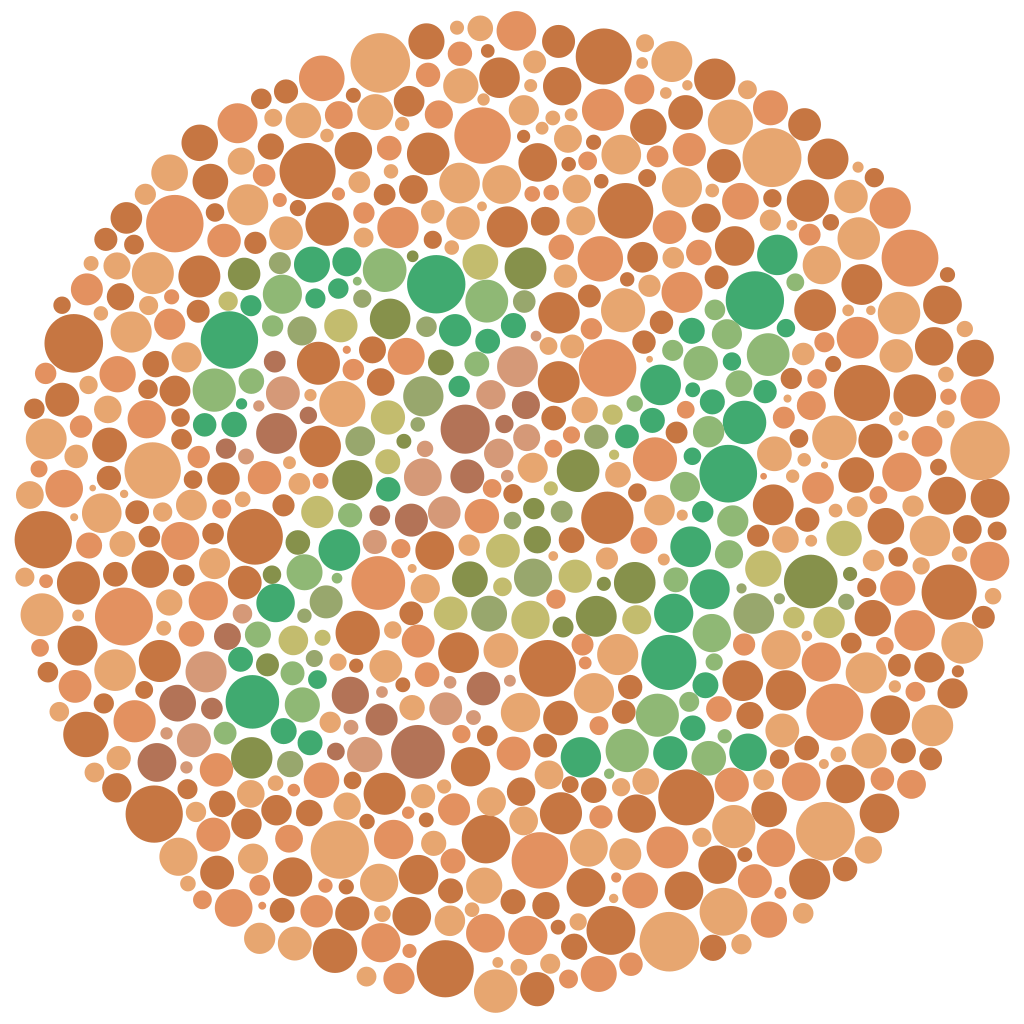
\includegraphics[width=0.3\textwidth]{Ishihara_9.png}
    \hspace{1cm}
    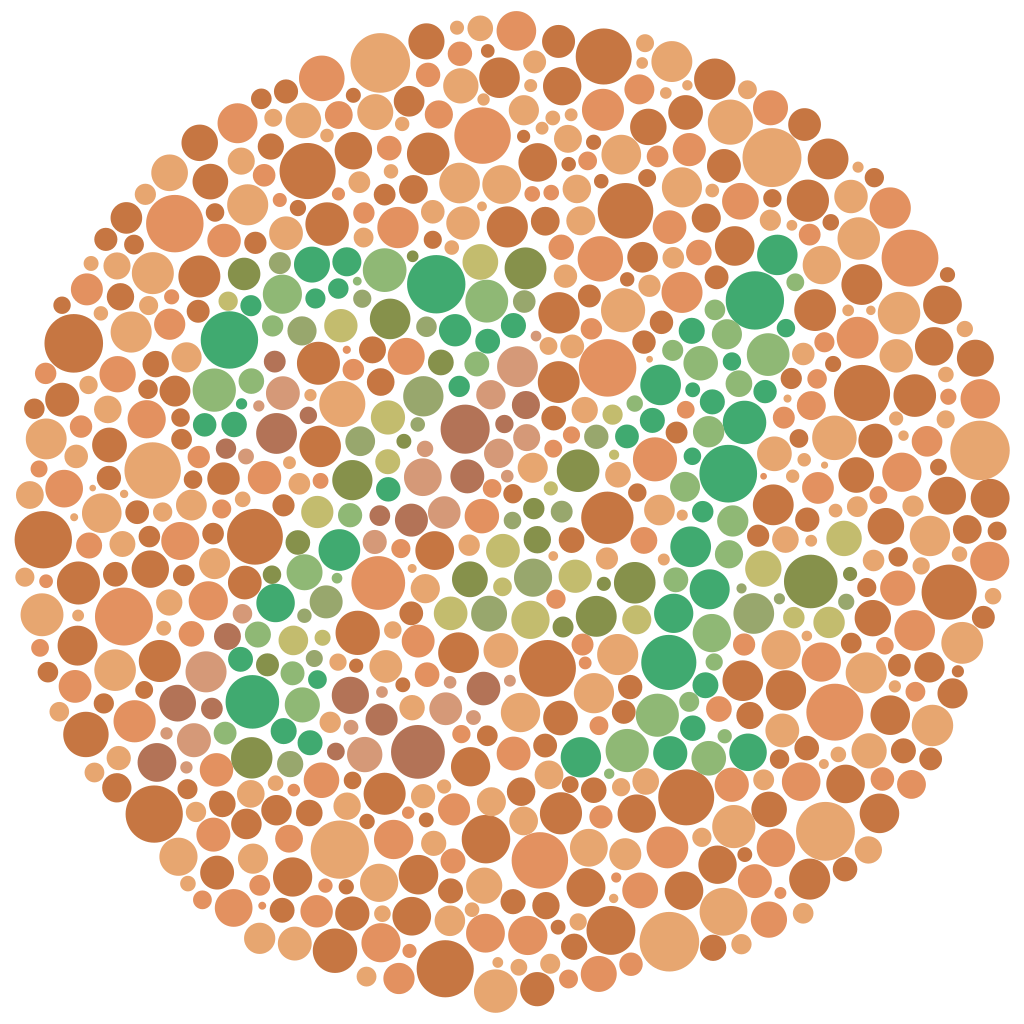
\includegraphics[decodearray={0 0 0 1 0 1}, width=0.3\textwidth]{Ishihara_9.png}
    \caption{Ishihara colorblindness test, normal vision and without the {\color{red}red} channel.}
\end{figure}

\printbibliography

\end{document}
